% Compiled with bundled Tectonic (XeTeX-compatible engine).
\documentclass[10pt,a4paper,fontset=none]{ctexart}

\usepackage[a4paper,left=19mm,right=19mm,top=18mm,bottom=19mm,headheight=14pt]{geometry}
\usepackage{fontspec}
\usepackage{xeCJK}
\setmainfont{Times New Roman}
\setsansfont{Arial}
\setmonofont{Menlo}[Scale=0.84]
\setCJKmainfont{Songti SC}
\setCJKsansfont{Heiti SC}
\setCJKmonofont{Songti SC}

\usepackage{amsmath}
\usepackage{unicode-math}
\setmathfont{STIX Two Math}
\usepackage{booktabs,longtable,tabularx,array}
\usepackage{enumitem}
\usepackage{xcolor}
\usepackage{tikz}
\usetikzlibrary{arrows.meta,positioning,fit,calc}
\usepackage{caption}
\usepackage{titlesec}
\usepackage{fancyhdr}
\usepackage{microtype}
\usepackage{hyperref}
\usepackage{bookmark}

\definecolor{DeepBlue}{HTML}{17365D}
\definecolor{Accent}{HTML}{2459A6}
\definecolor{SoftBlue}{HTML}{EAF1FB}
\definecolor{SoftGray}{HTML}{F4F6F8}
\definecolor{LineGray}{HTML}{D7DFEA}
\hypersetup{
  colorlinks=true,
  linkcolor=DeepBlue,
  citecolor=Accent,
  urlcolor=Accent,
  bookmarksnumbered=true,
  pdftitle={LLM MoE 架构演进：从稀疏路由到动态计算与通信结构重构},
  pdfauthor={Jiguo Li},
  pdfsubject={Large Language Model Mixture-of-Experts Architecture Survey},
  pdfkeywords={MoE, Routing, Load Balancing, Expert Parallelism, ScMoE}
}

\setlength{\parindent}{2em}
\setlength{\parskip}{2.5pt}
\setlength{\abovedisplayskip}{6pt}
\setlength{\belowdisplayskip}{6pt}
\setlength{\abovedisplayshortskip}{4pt}
\setlength{\belowdisplayshortskip}{4pt}
\setlength{\jot}{3pt}
\linespread{1.13}
\emergencystretch=2em
\setlist[itemize]{leftmargin=1.8em,itemsep=1pt,topsep=2pt,parsep=0pt}
\setlist[enumerate]{leftmargin=2em,itemsep=1pt,topsep=2pt,parsep=0pt}
\renewcommand{\arraystretch}{1.15}
\captionsetup{font=small,labelfont=bf,labelsep=quad}

\titleformat{\section}{\Large\bfseries\color{DeepBlue}}{\thesection}{0.7em}{}
\titleformat{\subsection}{\large\bfseries\color{DeepBlue}}{\thesubsection}{0.65em}{}
\titleformat{\subsubsection}{\normalsize\bfseries\color{DeepBlue}}{\thesubsubsection}{0.55em}{}
\titlespacing*{\section}{0pt}{14pt}{5pt}
\titlespacing*{\subsection}{0pt}{10pt}{3pt}
\titlespacing*{\subsubsection}{0pt}{7pt}{2pt}

\pagestyle{fancy}
\fancyhf{}
\fancyhead[L]{\small\color{gray}LLM MoE 架构演进}
\fancyhead[R]{\small\color{gray}\leftmark}
\fancyfoot[C]{\small\thepage}
\renewcommand{\headrulewidth}{0.3pt}

\newcolumntype{Y}{>{\raggedright\arraybackslash}X}
\newcolumntype{C}[1]{>{\centering\arraybackslash}p{#1}}
\newcommand{\term}[1]{\textbf{#1}}
\newcommand{\codeid}[1]{\textnormal{#1}}
\newcommand{\reported}{\textbf{论文报告：}}
\newcommand{\inference}{\textbf{本文判断：}}
\newcommand{\noteBox}[1]{%
  \begin{center}
  \fcolorbox{Accent}{SoftBlue}{\parbox{0.93\linewidth}{#1}}
  \end{center}}

\begin{document}

\begin{center}
  {\zihao{1}\bfseries\color{DeepBlue}
  LLM MoE 架构演进：从稀疏路由到动态计算与通信结构重构}\par
  \vspace{4pt}
  {\zihao{3}\color{DeepBlue} Expert Topology、Routing、Load Balance 与 Expert Parallel 的协同演化}\par
  \vspace{10pt}
  {\normalsize\textbf{Jiguo Li\footnote{本文在Codex协助下完成}}}\par
  \vspace{2pt}
  {\small\href{mailto:jiguolee@gmail.com}{jiguolee@gmail.com}}\par
  \vspace{6pt}
  {\small 2026 年 8 月}\par
\end{center}
\vspace{5pt}
\hrule

\begin{abstract}
Mixture-of-Experts（MoE）已经成为大语言模型在固定单 token 计算预算下扩展参数容量的核心架构之一。然而，若只按模型发布时间罗列 GShard、Switch、Mixtral、DeepSeekMoE、DeepSeek-V3 与新近动态 MoE，会掩盖真正推动结构变化的瓶颈迁移。本文综合算法、推理系统和高效架构三类 Survey，并回到代表性原始论文与官方技术报告，提出一个由五条耦合路线构成的统一框架：expert 粒度、expert 拓扑、路由自由度、负载均衡作用域和执行结构。基于该框架，本文把 MoE 演进归纳为八个演进节点；它们不是八代模型的线性年表，而是由六个主干节点与两个正交分支构成的依赖图。在历史时间轴之外，本文进一步用 Expert topology、Routing、Balance 和 Expert Parallel 四个控制面剖解任一代 MoE 的内部工作机制，分别回答“有哪些专家、每个 token 选谁、群体负载如何受控、选中的计算如何映射到设备”。最后给出适用于基座预训练的等预算实验设计、系统指标和仍待解决的研究问题。\textbf{核心结论是：现代 MoE 的竞争焦点已从“稀疏激活更多参数”转向“让语义路由、计算预算和物理执行解耦”。}
\end{abstract}

\noindent\textbf{关键词：}大语言模型；Mixture-of-Experts；稀疏路由；负载均衡；Expert Parallel；动态计算；ScMoE

\noteBox{\textbf{阅读提要：}第三章的八个节点描述历史上的瓶颈迁移；第四至七章则从 topology、routing、balance 和 Expert Parallel 四个控制面剖解单个 MoE 系统。前者是时间轴，后者是系统剖面，不能视为两套并列的“发展阶段”。}

\clearpage
\begingroup
\small
\setlength{\parskip}{0pt}
\linespread{1.02}\selectfont
\setcounter{tocdepth}{2}
\tableofcontents
\endgroup
\clearpage

\section{问题定义与分析范围}

经典 MoE 研究关注如何让 gating network 将样本分配给不同局部专家；LLM 时代的稀疏 MoE 则额外要求：总参数容量增长时，每个 token 的激活参数和计算量不能同比增长。现有三类综述分别提供互补视角：Cai 等人的 Survey 按算法、系统和应用建立全栈 taxonomy\cite{cai2024survey}；Liu 等人重点拆解推理阶段的模型、系统与硬件优化\cite{liu2024inference}; Zhu 等人则把 MoE 放回 sparse attention、SSM 和 hybrid architecture 的大图景中\cite{zhu2025speed}。本文不重复逐篇枚举，而是追问：\textbf{每一次结构变化消除了什么瓶颈，又把瓶颈转移到哪里？}

讨论范围限定为 decoder-only LLM 预训练中的稀疏 MoE，重点覆盖 FFN MoE，同时讨论会反向影响结构选择的 Expert Parallel（EP）、All-to-All、token capacity 与 expert placement。多模态 MoE、MoE-LoRA、外部模型 ensemble 和纯后训练专家融合不在本文范围内。模型能力数字只用于说明架构可扩展性，不能作为跨论文的因果比较：训练数据、token 数、优化器、上下文长度、post-training 和评测污染控制往往并不一致。

\section{统一形式化：MoE 同时优化什么}

\subsection{Token-choice MoE}

给定第 $t$ 个 token 的隐藏表示 $x_t\in\mathbf{R}^{d}$，Router 计算 expert affinity：
\begin{equation}
  s_{i,t}=\phi(x_t,e_i),\qquad
  \mathcal{K}_t=\operatorname{TopK}_{i\in\{1,\ldots,N\}}(s_{i,t}),
  \label{eq:router}
\end{equation}
其中 $N$ 是 routed experts 数，$e_i$ 是 expert routing embedding 或 Router 权重。输出为
\begin{equation}
  y_t=x_t+\sum_{i\in\mathcal{K}_t}g_{i,t}E_i(x_t),
  \qquad
  g_{i,t}=\frac{\exp(s_{i,t})}{\sum_{j\in\mathcal{K}_t}\exp(s_{j,t})}.
  \label{eq:moe}
\end{equation}
若存在 always-on shared experts，则在式~\eqref{eq:moe}中增加 $\sum_j E^{\mathrm{shared}}_j(x_t)$。从公式看，MoE 只是稀疏函数组合；从系统看，$\mathcal{K}_t$ 决定 token 要跨越哪些设备、每张卡获得多少 token，以及每个局部 GEMM 的形状。

\subsection{容量、质量与系统效率的三目标}

MoE 并不是单目标优化。粗略地，模型希望最大化总容量 $P_{\mathrm{total}}$，同时控制单 token 激活量 $P_{\mathrm{active}}$：
\begin{equation}
  P_{\mathrm{active}} \approx P_{\mathrm{dense}}
  +\frac{k}{N}P_{\mathrm{routed}}+P_{\mathrm{shared}},
  \label{eq:active}
\end{equation}
但式~\eqref{eq:active}只是参数口径近似：attention、embedding、shared experts、不同 expert 宽度及框架统计方式都会造成偏差。另一方面，令一个统计窗口内 expert $i$ 接收的 token 数为 $n_i$，则负载变异系数为
\begin{equation}
  \operatorname{CV}_{\mathrm{expert}}
  =\frac{\sqrt{\frac{1}{N}\sum_i(n_i-\bar n)^2}}{\bar n}.
  \label{eq:cv}
\end{equation}
低 CV 有利于 EP 吞吐，却不必然有利于知识 specialization。架构设计的根本张力是：\term{语义上允许不均匀，物理执行上又不能出现严重 straggler}。

\begin{table}[htbp]
\centering
\caption{决定 MoE 架构差异的六个问题}
\label{tab:sixquestions}
\small
\begin{tabularx}{\textwidth}{p{0.25\textwidth}Y}
\toprule
设计问题 & 典型选择 \\
\midrule
谁选择谁 & token-choice、expert-choice、balanced assignment、soft merging \\
激活多少专家 & fixed Top-1/2/8、threshold、adaptive-$k$、zero-compute slot \\
Expert 多大 & coarse homogeneous、fine-grained、tiny、heterogeneous size \\
是否有公共路径 & pure routed、shared expert、dense residual、cross-layer shortcut \\
在哪个范围均衡 & sequence、micro-batch、global batch、device、node、communication \\
谁处理运行时动态性 & auxiliary loss、router bias、capacity/drop、placement、结构保证 \\
\bottomrule
\end{tabularx}
\end{table}

\subsection{四个控制面：对象、决策、控制与执行}

表\ref{tab:sixquestions}中的设计问题并不处于同一层次。为了区分“历史上架构如何演进”和“一个具体 MoE 系统内部如何工作”，本文进一步按\term{状态变量、决策粒度和更新时间尺度}把系统横截面分为四个控制面：Topology 是较慢变化的模型结构；Routing 是逐 token 的离散决策；Balance 在一组 tokens 上统计并施加反馈；Expert Parallel（EP）把逻辑决策落实为设备上的通信与 kernel。第三章将沿历史时间轴讨论瓶颈迁移，第四至七章则分别展开这四个控制面；\textbf{后者不是四个新的发展阶段。}

形式上，可以把四层关系写成
\begin{align}
  \mathcal{E} &= T(\theta_{\mathrm{topo}}),
  &\text{Topology：构造 expert 集合、分组和共享关系}; \notag\\
  \mathcal{K}_t &= R(x_t,\mathcal{E};\theta_{\mathrm{route}},b),
  &\text{Routing：为 token $t$ 选择 expert 子集}; \notag\\
  n_i &= \sum_t \mathbf{1}[i\in\mathcal{K}_t],\quad
  (b,\alpha,c)\leftarrow C(\{n_i\},\pi),
  &\text{Balance：依据聚合负载更新 bias、loss 或 capacity}; \notag\\
  y_t &= \operatorname{EP}\!\left(x_t,\mathcal{K}_t,\pi,\sigma\right),
  &\text{EP：按 placement $\pi$ 和 schedule $\sigma$ 执行 dispatch/combine}. \label{eq:fourplanes}
\end{align}
其中 $\mathcal{E}$ 是逻辑 expert 集合，$\mathcal{K}_t$ 是 token 的路由结果，$n_i$ 是统计窗口内 expert $i$ 的负载，$b$、$\alpha$、$c$ 分别代表 Router bias、辅助损失强度和 capacity 控制量，$\pi$ 是 expert 到设备的映射，$\sigma$ 是通信与计算调度。式\eqref{eq:fourplanes}说明：四层并非独立模块，而是一个闭环。

\begin{figure}[htbp]
\centering
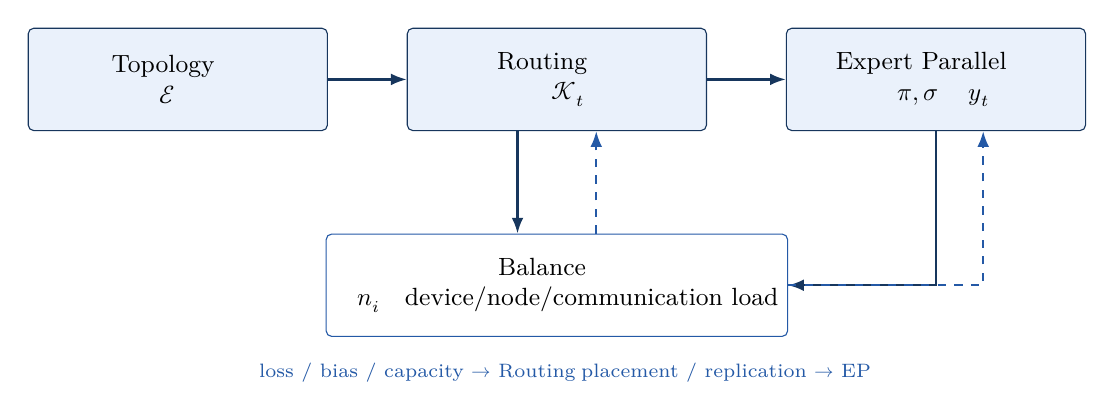
\begin{tikzpicture}[
  node distance=10mm and 10mm,
  plane/.style={draw=DeepBlue,rounded corners=2pt,fill=SoftBlue,minimum width=38mm,minimum height=13mm,align=center,font=\small},
  control/.style={draw=Accent,rounded corners=2pt,fill=white,minimum width=58mm,minimum height=13mm,align=center,font=\small},
  arr/.style={-{Latex[length=2mm]},thick,draw=DeepBlue},
  fb/.style={-{Latex[length=2mm]},thick,dashed,draw=Accent}
]
\node[plane] (topo) {Topology 对象层\\定义 $\mathcal{E}$ 与候选约束};
\node[plane,right=of topo] (route) {Routing 决策层\\输出 $\mathcal{K}_t$};
\node[plane,right=of route] (ep) {Expert Parallel 执行层\\按 $\pi,\sigma$ 输出 $y_t$};
\node[control,below=13mm of route] (bal) {Balance 控制层\\统计 $n_i$ 与 device/node/communication load};
\draw[arr] (topo)--(route);
\draw[arr] (route)--(ep);
\draw[arr] ([xshift=-5mm]route.south)--([xshift=-5mm]bal.north);
\draw[fb] ([xshift=5mm]bal.north)--([xshift=5mm]route.south);
\draw[arr] (ep.south) |- (bal.east);
\draw[fb] (bal.east) -| ([xshift=6mm]ep.south);
\node[font=\scriptsize\color{Accent},below=2mm of bal] {反馈：loss / bias / capacity $\rightarrow$ Routing；placement / replication $\rightarrow$ EP};
\end{tikzpicture}
\caption{Topology、Routing、Balance 与 Expert Parallel 的闭环关系。前三条实线形成前向执行链，虚线表示统计与系统代价对路由和放置的反馈。}
\label{fig:fourplanes}
\end{figure}

\begin{table}[htbp]
\centering
\caption{四个控制面的划分标准}
\label{tab:fourplanes}
\small
\begin{tabularx}{\textwidth}{>{\raggedright\arraybackslash}p{0.17\textwidth}>{\raggedright\arraybackslash}p{0.22\textwidth}>{\raggedright\arraybackslash}p{0.25\textwidth}Y}
\toprule
控制面 & 核心问题 & 主要状态与时间尺度 & 典型失败模式 \\
\midrule
Topology 对象层 & 有哪些 experts，它们多大、如何分组或共享 & 权重结构；架构设计/训练期慢变量 & 知识冗余、粒度过粗、共享路径过重 \\
Routing 决策层 & 当前 token 应选择哪些 experts、激活多少 & affinity、Top-$k$、候选约束；逐 token 快变量 & misrouting、离散优化困难、语义受拓扑约束 \\
Balance 控制层 & 一组 tokens 的使用分布是否满足训练和系统目标 & expert/device/node load；sequence 到 runtime 多尺度反馈 & collapse、过度均匀、straggler、通信热点 \\
Expert Parallel 执行层 & 选中的 expert 在何处、以何种通信和 kernel 执行 & placement、dispatch/combine、schedule；step/runtime 变量 & All-to-All 暴露、小 GEMM、P99 延迟、显存热点 \\
\bottomrule
\end{tabularx}
\end{table}

四层之间存在两类不能忽略的反向依赖。第一，物理拓扑会约束语义路由：device-limited routing 为降低 fan-out，主动缩小 $\mathcal{E}$ 中对某个 token 可见的候选集合。第二，Balance 不只调 Router：runtime replication 或 expert placement 可以在不改变 $\mathcal{K}_t$ 的情况下改善物理负载。因此“负载均衡”不能只理解为一个 auxiliary loss，“Expert Parallel”也不是模型结构确定后才介入的被动实现。

\section{八个演进节点：划分标准、主干与分支}

这里的“八个”不是从某篇 Survey 直接摘录的固定 taxonomy，也不是按年份机械切段，而是本文依据\term{主导瓶颈迁移}做出的分析性归纳。一个变化只有同时满足以下三点，才被单列为演进节点：第一，它引入了可独立调节的新设计变量，例如 Top-$k$、expert 粒度、shared path 或动态 active budget；第二，它使系统的主要矛盾发生迁移，例如从计算随 expert 数线性增长，转为离散路由与负载不均，再转为 All-to-All、小 GEMM 或权重 I/O；第三，它被后续架构继承，因而不是某个模型的一次性实现细节。

按这一标准，节点 1--6 构成较清晰的历史主干：统计分工 $\rightarrow$ 稀疏激活 $\rightarrow$ Transformer 规模化 $\rightarrow$ decoder-only 产品化 $\rightarrow$ 细粒度知识组织 $\rightarrow$ ultra-sparse 容量扩展。节点 7 和节点 8 则不是简单接在节点 6 之后的新“代际”：节点 7 放松“每个 token 固定计算量”的假设；节点 8 放松“语义路由、层内 expert 拓扑和物理通信必须绑定”的假设。二者都可与节点 5 或 6 的 expert 结构组合。图\ref{fig:evolution-dag}给出这种继承关系。

\begin{figure}[htbp]
\centering
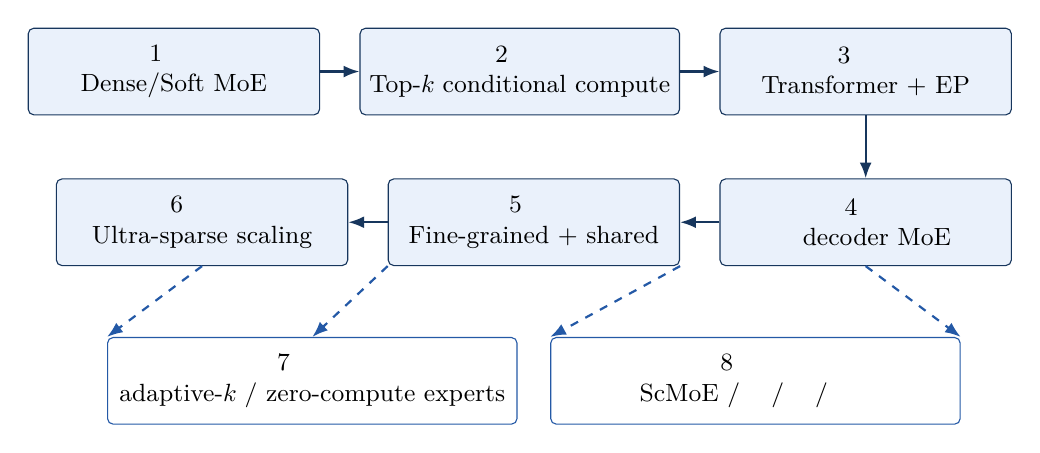
\begin{tikzpicture}[
  node distance=5mm and 5mm,
  stage/.style={draw=DeepBlue,rounded corners=2pt,fill=SoftBlue,minimum width=37mm,minimum height=11mm,align=center,font=\small},
  branch/.style={draw=Accent,rounded corners=2pt,fill=white,minimum width=52mm,minimum height=11mm,align=center,font=\small},
  arr/.style={-{Latex[length=2mm]},thick,draw=DeepBlue},
  darr/.style={-{Latex[length=2mm]},thick,dashed,draw=Accent}
]
\node[stage] (s1) {1 统计分工\\Dense/Soft MoE};
\node[stage,right=of s1] (s2) {2 稀疏激活\\Top-$k$ conditional compute};
\node[stage,right=of s2] (s3) {3 集群规模化\\Transformer + EP};
\node[stage,below=8mm of s3] (s4) {4 产品化\\开放 decoder MoE};
\node[stage,left=of s4] (s5) {5 知识细分\\Fine-grained + shared};
\node[stage,left=of s5] (s6) {6 容量继续扩展\\Ultra-sparse scaling};
\node[branch,below=9mm of s6,xshift=14mm] (s7) {7 计算预算动态化\\adaptive-$k$ / zero-compute experts};
\node[branch,below=9mm of s4,xshift=-14mm] (s8) {8 语义与物理解耦\\ScMoE / 异构 / 跨层 / 结构化通信};
\draw[arr] (s1)--(s2);
\draw[arr] (s2)--(s3);
\draw[arr] (s3)--(s4);
\draw[arr] (s4)--(s5);
\draw[arr] (s5)--(s6);
\draw[darr] (s5.south west)--(s7.north);
\draw[darr] (s6.south)--(s7.north west);
\draw[darr] (s5.south east)--(s8.north west);
\draw[darr] (s4.south)--(s8.north east);
\end{tikzpicture}
\caption{八个演进节点的关系。实线表示历史主干上的主要继承，虚线表示可叠加的正交分支；节点编号不代表严格代际替换。}
\label{fig:evolution-dag}
\end{figure}

\begin{table}[htbp]
\centering
\caption{八个节点的划分依据与瓶颈迁移}
\label{tab:evolution-nodes}
\small
\begin{tabularx}{\textwidth}{p{0.055\textwidth}p{0.18\textwidth}p{0.25\textwidth}Y}
\toprule
节点 & 新增设计变量 & 解决的主导问题 & 转移出的新瓶颈 \\
\midrule
1 & gating 与 expert specialization & 单模型难以对输入空间分区建模 & 所有 experts 都计算，容量与 FLOPs 绑定 \\
2 & 稀疏 Top-$k$ 与 capacity & total parameters 与 active FLOPs 解耦 & 离散路由、collapse、token drop \\
3 & EP、All-to-All、稳定化 loss & Transformer MoE 的集群级训练 & 通信、straggler、数值与负载稳定性 \\
4 & decoder-only 训练与部署闭环 & 证明经典 MoE 可进入开放模型生态 & 大 expert 知识冗余、组合粒度粗 \\
5 & fine-grained、shared、device limit & 公共知识重复与专家组合不足 & fan-out、小 GEMM、共享路径固定成本 \\
6 & 更大 $N$、tiny experts、检索式路由 & 固定 active budget 下继续扩 total capacity & 权重 I/O、检索、低 token/expert \\
7 & adaptive compute / zero slots & token 难度不同却使用固定 Top-$k$ & active budget 控制、尾延迟、训练稳定性 \\
8 & shortcut、异构/跨层拓扑、结构化通信 & 语义路由被设备拓扑和通信绑定 & 调度复杂度、缓存一致性、大规模验证 \\
\bottomrule
\end{tabularx}
\end{table}

\subsection{Dense/Soft MoE：统计分工而非计算稀疏}

Jacobs 等人在 1991 年提出 gating network 与 local experts 的基本形式\cite{jacobs1991adaptive}。这一节点建立的是\term{统计分工}：gate 根据输入产生混合权重，不同子网络拟合输入空间的不同区域，训练目标可以推动 specialization。由于所有 experts 通常都参与加权，路由是连续可导的，既不需要 token capacity，也不存在 All-to-All 意义上的稀疏 dispatch。

\textbf{为什么单列。}它定义了后来 MoE 一直保留的三个角色：Router/gate、experts 和 weighted combine。\textbf{为何还不是现代稀疏 MoE。}增加 expert 数会近似线性增加计算，因此“模型容量”和“每 token FLOPs”尚未解耦。节点 2 继承其统计分工目标，但将 dense mixture 改为只执行少数 experts；这一步才产生 conditional scaling，也同时产生离散选择带来的训练与系统问题。

\subsection{Sparse conditional computation：Top-k 建立容量杠杆}

Shazeer 等人将 noisy Top-$k$ routing 用于超大稀疏网络\cite{shazeer2017outrageously}，使每个输入只执行少数 experts。若总 expert 数为 $N$、每个输入只激活 $k\ll N$ 个 experts，那么 total capacity 可以随 $N$ 增长，而主要 expert FLOPs 近似只随 $k$ 增长。这里第一次形成现代 MoE 的容量杠杆：\term{参数容量与单 token 计算量解耦}。

这一解耦并非免费。Top-$k$ 使未选 expert 没有来自该 token 的梯度；热门 experts 会溢出 capacity，冷门 experts 可能长期得不到训练；跨设备执行还必须加入 dispatch/combine。因而 noisy routing、importance/load auxiliary loss、capacity factor 和 token drop 不是外围技巧，而是稀疏执行本身诱发的配套机制。节点 3 并不改变这一基本算法，而是回答：当 MoE 被反复嵌入 Transformer 层、扩展到数千设备时，如何让它稳定且可执行。

\subsection{Transformer MoE 与 Expert Parallel}

GShard 将 Top-2 MoE FFN 系统化嵌入 Transformer，并依靠自动 sharding 在\textbf{2048 个 TPU}上训练\textbf{超过 600B}的多语言模型\cite{lepikhin2020gshard}。经典执行链由此固定为
\begin{center}
\textsf{Attention $\rightarrow$ Router $\rightarrow$ Dispatch All-to-All $\rightarrow$ Expert FFN $\rightarrow$ Combine All-to-All}.
\end{center}
这一节点的新增变量不是“更多 experts”，而是\term{expert parallelism 与集群执行语义}：token 如何跨设备重排、每个 expert 如何批处理、溢出如何处理、通信与计算如何同步。Switch Transformer 进一步采用 Top-1，以更低通信和更简单的执行换取专家组合能力与路由容错下降\cite{fedus2021switch}。ST-MoE 则把稳定性提升为一等设计目标，引入 Router z-loss 约束 logits 数值尺度\cite{zoph2022stmoe}。需要区分：z-loss 控制数值稳定，balance loss 控制使用分布，两者不是同一机制。

同期，BASE Layers 把训练路由写成严格均衡的线性分配问题\cite{lewis2021base}，Expert Choice 则让 experts 选择固定容量 tokens\cite{zhou2022expertchoice}。它们能够直接保证均衡，但 batch-level 联合分配和 expert-side capacity 对在线自回归 decoding 不如 token-choice 自然，因此没有取代 decoder-only LLM 的 Top-$k$ 主干。节点 3 的遗产是“Router + EP + capacity/balance + All-to-All”这一完整系统契约；节点 4 和 5 都沿用它，只是把重点从“能否大规模训练”转向模型质量、部署可用性和 expert 内部组织。

\subsection{开放权重 coarse-grained MoE}

Mixtral 采用\textbf{8$\times$7B、每 token Top-2}\cite{jiang2024mixtral}。它没有发明新的 Router family，因此若只按算法新颖性看，似乎不应成为独立节点。但它补齐了另一条关键证据链：\term{经典 coarse-grained MoE 可以在开放权重 decoder-only LLM 中贯通预训练、指令微调、推理部署与社区复现}。

\textbf{为什么单列。}节点 3 证明的是超大集群上的训练可扩展性；节点 4 证明的是通用 decoder 模型的可用性和部署闭环。它继承 Top-$k$、同构 experts 和 EP，不改变基本执行链。也正因为系统已能稳定运行，主要矛盾才显露为知识组织问题：少量大 experts 容易重复学习公共能力，Router 只能在很粗的知识块之间组合。节点 5 正面处理这一瓶颈。

\subsection{Shared + fine-grained experts}

DeepSeekMoE 对粗粒度专家做了两项关键改造\cite{dai2024deepseekmoe}：其一，把一个大 FFN 切成多个较小 experts，使 Router 在相同 active budget 下组合更多知识单元；其二，加入 shared expert isolation，把所有 token 都需要的公共知识交给 always-on 路径，减少 routed experts 的知识冗余。前者提高\term{组合分辨率}，后者把“公共能力”和“条件能力”显式拆开。DeepSeek-V2 将这一结构扩大到\textbf{236B/21B active}，并加入 device-limited routing：每个 token 的候选 experts 被限制在少量设备内，从而控制跨设备 fan-out\cite{deepseekv2}。

共享或稠密路径还能提供隐藏通信的计算窗口。DeepSeek-V2 将 shared expert computation 与 EP communication overlap；Snowflake Arctic 的 dense residual path 也体现了同类算法--系统协同\cite{snowflakearctic}。但\term{shared expert 不是 fine-grained MoE 的必要条件}。Qwen3-235B-A22B 采用\textbf{128 个细粒度 experts、Top-8}，却移除 shared expert，并依靠 global-batch balance 允许常用能力在 routed experts 中自然形成\cite{qwen3}。

因此，节点 5 实际包含两个可拆分的轴：expert granularity 与 shared path。它们经常组合，但不存在逻辑绑定。节点 5 继承节点 3 的 EP 系统，却把 expert 数、Top-$k$ 和设备 fan-out 同时推高，使小 GEMM、路由碎片化和通信拓扑成为新瓶颈。节点 6 沿着“更多、更小 experts”继续扩展；节点 8 则试图改变 fan-out 与通信的物理实现。

\subsection{Ultra-sparse scaling}

这一阶段的问题变为：\emph{固定 active parameters 时，继续增加 total experts 是否仍能降低 loss？}PEER 用 product-key retrieval 从\textbf{超过百万个 tiny experts}中选择少数 experts\cite{he2024peer}；Kimi K2 将工程可落地的 ultra-sparse 结构扩展到\textbf{1.04T/32.6B active、384 routed experts、Top-8}，并报告固定 active budget 下更高 sparsity 的 scaling 收益\cite{kimiK2}；gpt-oss-120b 则采用\textbf{128 experts、Top-4}和较小 active footprint，体现面向本地部署的高稀疏路线\cite{openaiGptOss}。

\textbf{为什么从 fine-grained 单列。}fine-grained 的首要目标是减少知识冗余、提高组合分辨率；ultra-sparse 的首要问题则是 scaling：固定 active parameters 和训练 FLOPs 时，扩大候选 expert 集是否持续改善 loss。二者都增加 expert count，但优化目标不同。

\term{稀疏度不能无限增加。}随着 $N$ 增大，Router scoring、expert weight I/O、All-to-All metadata 和小 GEMM 碎片化都会上升；当每个 expert 每步获得的 tokens 太少时，\textbf{理论 FLOPs 优势不能转化为 wall-clock 收益}。这意味着节点 6 没有终结节点 5，反而更依赖其 fine-grained 组织和路由控制。节点 7 与 8 则从两个正交方向绕开固定 Top-$k$ 主干的限制。

\subsection{动态计算：从固定 Top-k 到 token-dependent budget}

固定 Top-$k$ 隐含所有 token 使用相同数量的 expert FLOPs，即便 token 的语义难度和所需容量不同。LongCat-Flash 加入 zero-computation experts：Router 仍选择固定 slots，但部分 slots 是 identity，因此真实执行的 FFN 数量随 token 变化\cite{longcatFlash}。adaptive-$k$、threshold routing 与 zero-compute slots 的共同目标，是\term{把“选哪个 expert”和“到底计算多少”从一个固定超参数中拆开}。

\textbf{与节点 6 的关系。}ultra-sparse 扩大的是候选容量 $N$，但通常仍保持固定 $k$；动态计算改变的是每个 token 的实际 $k_t$ 或有效 FFN 数。两者可以组合：候选池很大，同时简单 token 少算、困难 token 多算。控制目标也由单一 expert load 扩展为“平均 active budget + budget variance + real-expert load + P99 latency”。训练时的平均 FLOPs 约束并不能自动保证在线尾延迟，因为困难 tokens 可能在同一 micro-batch 或请求窗口内聚集。

动态计算的遗留问题是闭环控制：若 Router 同时决定语义 expert 和计算预算，balance bias 既影响 specialization，又影响吞吐；若只约束长期均值，又可能出现短时 burst。因而 adaptive bias/PID 式反馈、budget loss 与 runtime admission control 是配套问题，而非单纯修改 Top-$k$ 即可解决。

\subsection{语义路由与物理执行解耦}

节点 1--7 主要改变 Router 可选的专家或 active budget；节点 8 改变的是更底层的假设：\term{语义上选中了某个 expert，并不意味着必须沿固定的层内 All-to-All 路径立即执行它}。这一节点不是单一模型家族，而是四条具有共同目标的前沿分支。

\textbf{执行依赖重排。}ScMoE 不改变 token 选哪些 experts，而是改变依赖图。其跨层 shortcut 让 routed experts 消费前层中间表示，同时用当前 dense/shared path 覆盖 dispatch/combine 的通信窗口\cite{cai2024scmoe}。它解决的是 exposed communication，不直接解决 routing skew。图\ref{fig:scmoe}给出抽象比较。

\begin{figure}[htbp]
\centering
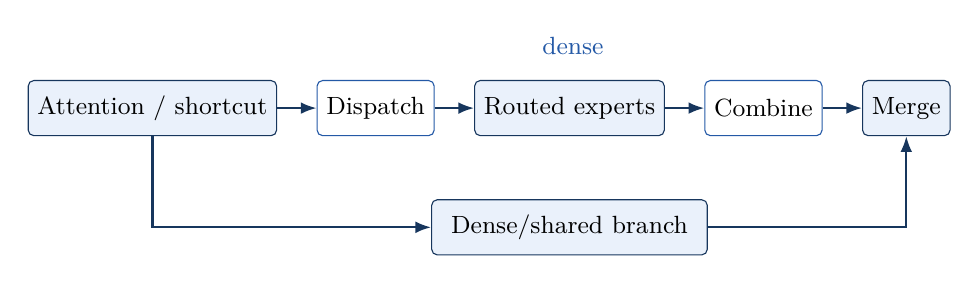
\begin{tikzpicture}[
  node distance=5mm and 5mm,
  box/.style={draw=DeepBlue,rounded corners=2pt,fill=SoftBlue,minimum height=7mm,align=center,font=\small},
  comm/.style={draw=Accent,rounded corners=2pt,fill=white,minimum height=7mm,align=center,font=\small},
  arr/.style={-{Latex[length=2mm]},thick,draw=DeepBlue}
]
\node[box] (attn) {Attention / shortcut};
\node[comm,right=of attn] (dispatch) {Dispatch};
\node[box,right=of dispatch] (expert) {Routed experts};
\node[comm,right=of expert] (combine) {Combine};
\node[box,right=of combine] (merge) {Merge};
\node[box,below=8mm of expert,minimum width=35mm] (dense) {Dense/shared branch};
\draw[arr] (attn)--(dispatch);
\draw[arr] (dispatch)--(expert);
\draw[arr] (expert)--(combine);
\draw[arr] (combine)--(merge);
\draw[arr] (attn.south) |- (dense.west);
\draw[arr] (dense.east) -| (merge.south);
\node[font=\small\color{Accent},above=2mm of expert] {通信路径与 dense 计算并行};
\end{tikzpicture}
\caption{ScMoE 的核心是重排执行依赖以扩大通信隐藏窗口；它不是新的路由算法。}
\label{fig:scmoe}
\end{figure}

LongCat-Flash 将 ScMoE 与 token-dimension chunking、Single Batch Overlap 结合；LongCat-2.0 的官方报告进一步在专用 accelerator 上采用 dense/MoE per-core full parallel execution\cite{longcat2}。这些进展降低 exposed communication，\textbf{但不会自动解决严重 routing skew、expert 内部计算差异和显存压力}。

\textbf{异构 expert。}MoHGE 采用两级路由：先选 expert group，再在组内选择不同大小 experts，并结合 group-wise 与 intra-group balance 约束部署\cite{mohge2026}。它把“expert 等宽”从默认约束变成设计变量，使不同 token 可获得不同形态的计算能力；代价是异构 GEMM、容量规划和负载指标都更复杂。

\textbf{跨层共享。}GMoE 把一部分 experts 设为跨层共享的 Global Experts，同时保留 layer-local experts，以减少跨层能力冗余\cite{gmoe2026}。这与 shared expert 的区别在于共享作用域：前者跨 layer，后者通常是在单层内对所有 tokens always-on。跨层共享会引入缓存、调度和层间干扰问题。

\textbf{结构化通信。}Multi-Head LatentMoE 与 Head Parallel 尝试改变通信拓扑，使通信量相对 activated expert 数 $k$ 为 $O(1)$，并获得更确定的流量\cite{cui2026latentmoe}。与 ScMoE“隐藏动态通信”不同，这条路线试图“减少或结构化通信本身”。由于尚缺少 trillion-parameter、万卡级公开验证，\term{它应被视为研究前沿，而非已经替代 Top-$k$ EP 的主流}。

四条分支分别优化时间重叠、计算形态、参数复用和数据移动，可组合而非替代。

\section{Expert topology：对象层}

在第二章的四层框架中，Topology 是对象层：它先定义 expert 集合 $\mathcal{E}$、知识单元的粒度、共享范围和计算异质性，Routing 才能在其上做逐 token 选择。因而，Topology 的核心不只是 expert count，而是\term{Router 可以组合什么样的计算单元}。

把 MoE 演进只理解为 expert count 增长是不充分的。表\ref{tab:topology}显示，真正变化的是知识单元的粒度、共享范围和计算异质性。

\begin{table}[htbp]
\centering
\caption{Expert topology 的主要演进路线}
\label{tab:topology}
\small
\begin{tabularx}{\textwidth}{p{0.21\textwidth}p{0.23\textwidth}Y Y}
\toprule
拓扑 & 代表工作 & 主要收益 & 新瓶颈 \\
\midrule
少量同构大专家 & GShard、Switch、Mixtral & 实现 conditional scaling & 知识重复、组合性有限 \\
Shared/dense + routed & DeepSeekMoE、Arctic & 公共知识隔离，可制造 overlap window & 固定 FLOPs 增加，公共路径可能过重 \\
Fine-grained experts & DeepSeek-V2/V3、Qwen3 & 更细知识组合，更高 total/active ratio & 路由、通信与 GEMM 更碎 \\
Ultra-sparse experts & PEER、Kimi K2、gpt-oss & 固定 FLOPs 下继续扩容量 & 检索、权重 I/O、低 token/expert \\
Heterogeneous/dynamic & LongCat、MoHGE & token 级动态计算预算 & budget control 与物理均衡耦合 \\
Cross-layer global/local & GMoE & 减少跨层 expert 冗余 & 调度、缓存与层间干扰待验证 \\
Latent/head structured & Multi-Head LatentMoE & 通信确定化、与 $k$ 解耦 & 大规模质量证据不足 \\
\bottomrule
\end{tabularx}
\end{table}

另一个经常被忽略的维度是初始化方式。Sparse Upcycling 将已有 dense FFN 复制成多个 experts，再新增 Router 继续训练\cite{komatsuzaki2022upcycling}。它复用 dense checkpoint，却带来 expert symmetry，需要路由噪声、数据差异和后续训练使 experts 分化。更进一步的 Expert Upcycling 从已有 $E$-expert MoE 扩展到 $mE$ experts，同时保持 Top-$k$ 与 active cost 不变\cite{expertUpcycling2026}。upcycling 不是新的 Router family，但会改变 specialization 的形成路径和训练成本。

\section{Routing：决策层}

在图\ref{fig:fourplanes}的闭环中，Routing 接收 Topology 定义的 expert 集合与系统施加的候选约束，对每个 token 产生 $\mathcal{K}_t$。它优化的是\term{局部语义匹配}，并不直接保证一个 sequence、batch 或 device 上的总体负载合理；后者属于第六章的控制层。

\begin{table}[htbp]
\centering
\caption{主要 Router family 及其适用边界}
\label{tab:router}
\small
\begin{tabularx}{\textwidth}{p{0.24\textwidth}p{0.19\textwidth}Y Y}
\toprule
Router family & 决策单位 & Balance 特性 & decoder-only LLM 适用性 \\
\midrule
Noisy Top-$k$ token-choice & token 选 experts & 需 loss、bias 或 runtime 均衡 & 当前主干，在线自然 \\
Top-1 Switch & token 选 1 expert & 通信简单，capacity 更敏感 & 可扩展，但组合能力受限 \\
Balanced assignment & batch 联合分配 & 训练时严格等量 & 全局求解复杂，在线不自然 \\
Expert-choice & expert 选 tokens & expert 容量天然固定 & encoder 更自然，decoder capacity 难处理 \\
Soft/parameter merging & 连续混合 & 可微、无离散 Top-$k$ & 大规模 EP 效率尚未证明 \\
Bias-controlled Top-$k$ & affinity + 非梯度 bias & 不把均衡梯度写入 LM 参数 & DeepSeek-V3 等模型采用 \\
Zero experts/adaptive-$k$ & token 计算量可变 & 需约束平均预算与尾部 & 动态计算的重要方向 \\
\bottomrule
\end{tabularx}
\end{table}

Token-choice 成为主流并不表示它在优化上最优，而是它最符合自回归在线约束：当前 token 的路由只依赖当前状态，不需要等待未来 tokens 或求解整个 batch 的全局分配。Soft MoE 和 Lory 等连续路由方案避免离散 Top-$k$，但尚未在超大规模 decoder 与低延迟 EP 上证明系统优势\cite{puigcerver2023softmoe,zhong2024lory}。

路由自由度还受到网络拓扑约束。device-limited 或 node-limited routing 将候选 expert 限制在少量设备/节点集合，降低单 token 的通信 fan-out。代价是语义最优 expert 可能被拓扑约束排除，因此这类设计本质上是质量与通信之间的显式折中。

\section{Balance：控制层}

Balance 不重新定义 experts，也不独立生成 token 的语义路由。它观察许多次 Routing 决策累积出的 $\{n_i\}$ 及设备、节点和通信负载，再通过 loss、bias、capacity 或 runtime placement 反馈给决策层和执行层。其核心问题是：\term{允许语义 specialization 不均匀的同时，如何避免训练 collapse 和物理 straggler}。

\subsection{Sequence/batch-wise expert balance}

经典辅助损失可写为
\begin{equation}
  \mathcal{L}_{\mathrm{bal}}=\alpha N\sum_{i=1}^{N} f_i P_i,
  \label{eq:balance}
\end{equation}
其中 $f_i$ 是统计窗口内实际分配到 expert $i$ 的 token fraction，$P_i$ 是平均 routing probability，$\alpha$ 控制均衡强度。当所有 experts 使用近似均匀时，式~\eqref{eq:balance}较小。该损失同时承担防止 expert collapse 和避免 EP straggler 两项职责，但二者并不等价：模型可能需要不均匀 specialization，硬件却希望均匀负载。$\alpha$ 过大时，硬件目标会直接干扰语言建模梯度。

\subsection{Device/node/communication-aware balance}

DeepSeek-V2 把 balance 拆为 expert-level、device-level 与 communication balance，并通过 device-limited routing 控制 fan-out\cite{deepseekv2}。这一变化的关键不是多加几个 loss，而是承认\term{逻辑 expert 均衡不等于物理设备或网络均衡}：若一个 device 上有多个 experts，只要 device 间总 token 接近，未必需要所有 experts 完全等量。

\subsection{Auxiliary-Loss-Free Load Balancing}

Auxiliary-Loss-Free（ALF）策略给每个 expert 增加非梯度 routing bias $b_i$：
\begin{equation}
  \mathcal{K}_t=\operatorname{TopK}_i(s_{i,t}+b_i),\qquad
  b_i\leftarrow b_i+\eta\,\operatorname{sign}(\bar n-n_i),
  \label{eq:alf}
\end{equation}
其中 $\eta$ 是 bias 更新速度。bias 影响 Top-$k$ 选择，但不作为 affinity 权重参与 LM 梯度，从而减少均衡目标对模型参数更新方向的直接干扰\cite{wang2024auxfree}。DeepSeek-V3 使用 batch-wise ALF 作为主均衡机制，同时保留很弱的 sequence-wise auxiliary loss，防止单序列极端失衡\cite{deepseekv3}。因此，\term{“DeepSeek-V3 完全没有任何 balance loss”并不准确}。

global-batch 统计比单 micro-batch 更稳定，也允许某些 experts 在局部 batch 上承载更多特定 domain token；代价是需要跨 DP/EP 范围聚合负载，扩大统计范围可能引入额外通信。

\subsection{Runtime expert placement}

训练分布上的均衡不能保证真实推理流量。domain shift、SFT/RL 和关闭 balance 更新都会改变 expert popularity。DeepSeek-V3 使用冗余 expert deployment，在运行时复制热点 experts 并调整 placement\cite{deepseekv3}。这一趋势把目标重新分工：Router 可以保留语义上的非均匀 specialization，runtime 通过复制、迁移或重新放置避免设备 straggler。

\begin{figure}[htbp]
\centering
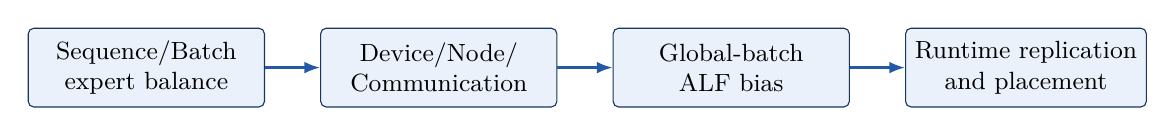
\begin{tikzpicture}[
  stage/.style={draw=DeepBlue,fill=SoftBlue,rounded corners=2pt,minimum width=30mm,minimum height=10mm,align=center,font=\small},
  arr/.style={-{Latex[length=2mm]},thick,draw=Accent}
]
\node[stage] (s1) {Sequence/Batch\\expert balance};
\node[stage,right=7mm of s1] (s2) {Device/Node/\\Communication};
\node[stage,right=7mm of s2] (s3) {Global-batch\\ALF bias};
\node[stage,right=7mm of s3] (s4) {Runtime replication\\and placement};
\draw[arr] (s1)--(s2);
\draw[arr] (s2)--(s3);
\draw[arr] (s3)--(s4);
\end{tikzpicture}
\caption{Balance 的演进不是简单减弱约束，而是逐步把物理执行目标从 LM 梯度中剥离。}
\label{fig:balance}
\end{figure}

\section{Expert Parallel：执行层}

EP 消费 Routing 产生的 token--expert assignment，并结合 placement $\pi$ 把逻辑 expert 转化为设备上的 dispatch、局部 GEMM 与 combine。它通常不改变“语义上选中了谁”，却决定这次选择的 wall-clock 成本；当系统代价过高时，又会通过 device-limited routing、placement 或架构重构反向修改前三层。

MoE 的算法收益只有在稀疏执行高效时才成立。capacity-based 系统为每个 expert 预留固定 token slots，溢出 token 被丢弃或走 residual，容易造成训练与推理不一致。MegaBlocks 使用 block-sparse kernels 实现 dropless MoE，使动态 token shape 不再要求 token dropping\cite{gale2022megablocks}。Tutel 等系统则动态选择并行和 pipeline 策略，以适配不同集群规模\cite{hwang2022tutel}。

随着专家更细、Top-$k$ 更大，通信逐渐成为一等架构约束，推动出三种处理方式：
\begin{enumerate}
  \item \term{限制通信拓扑}：device/node-limited routing 降低 fan-out；
  \item \term{隐藏通信}：shared computation overlap、DualPipe、ScMoE 和 token chunking 扩大 overlap window；
  \item \term{重构通信}：Head Parallel 等方案把动态流量变为更确定的通信模式。
\end{enumerate}

这里\term{必须区分“总 All-to-All 时间”和“exposed communication time”}。若通信完全被 dense path 覆盖，继续优化链路带宽对端到端 step time 的边际收益会下降；反之，即使总通信量不变，只要关键路径缩短，吞吐也可能显著改善。因此训练报告至少应同时给出\textbf{通信量、overlap 比例、exposed dispatch/combine、MFU 和 step-time P99}。

\section{现代主干与前沿分支}

截至 2026 年，大规模 decoder MoE 最常见的组合可概括为：
\begin{center}
\fcolorbox{DeepBlue}{SoftGray}{\parbox{0.88\textwidth}{\centering
Token-choice Top-$k$ + fine-grained experts + 可选 shared path + global/batch-wise balance 或 ALF + topology-limited routing + dropless kernels/communication overlap + runtime expert placement}}
\end{center}

DeepSeek-V3、Qwen3 和 Kimi K2 在 shared expert、balance 机制和 EP size 上不同，但都位于这条主干。与此同时，以下分支仍未形成统一结论：
\begin{itemize}
  \item \term{MoE Attention}：JetMoE 同时稀疏化 Attention 与 FFN，进一步降低 active FLOPs，但 KV/cache 和路由更复杂\cite{shen2024jetmoe}；
  \item \term{Hybrid mixer + MoE}：Jamba 在 Transformer 与 Mamba layers 间交替，说明 MoE 是参数扩容方式，不绑定全 Attention backbone\cite{lieber2024jamba}；
  \item \term{Million experts}：理论组合性高，但权重 I/O、小 GEMM 和检索开销仍限制工业部署；
  \item \term{Heterogeneous experts}：按 token 难度选择不同容量，表达自然，但物理放置和尾延迟更难；
  \item \term{Cross-layer global experts}：目标是消除层间重复能力，仍缺少超大规模训练证据；
  \item \term{Structured communication}：Head Parallel 可能降低动态 EP 痛点，但尚处早期验证阶段。
\end{itemize}

表\ref{tab:models}以架构选择而非 benchmark 排名对代表性模型进行对照。

\begin{table}[htbp]
\centering
\caption{代表性 LLM MoE 的架构位置；active 参数口径因报告而异}
\label{tab:models}
\scriptsize
\begin{tabularx}{\textwidth}{p{0.18\textwidth}C{15mm}C{25mm}C{22mm}Y}
\toprule
模型 & 年份 & Total/Active & Experts/Top-$k$ & 架构意义 \\
\midrule
GShard & 2020 & $>$600B/未统一披露 & Top-2 & Transformer MoE 与自动 sharding \\
Switch & 2021 & up to 1T+ & Top-1 & 用简单路由换吞吐与可扩展性 \\
Mixtral 8$\times$7B & 2024 & 46.7B/12.9B & 8/2 & 开放 coarse-grained MoE 标杆 \\
DeepSeek-V2 & 2024 & 236B/21B & 160/6 & fine-grained、shared、device-limited \\
DeepSeek-V3 & 2024 & 671B/37B & 256/8 & ALF、weak seq loss、node-limited \\
Qwen3-235B-A22B & 2025 & 235B/22B & 128/8 & fine-grained、无 shared、global balance \\
Kimi K2 & 2025 & 1.04T/32.6B & 384/8 & ultra-sparse scaling \\
gpt-oss-120b & 2025 & 116.8B/5.1B & 128/4 & 小 active footprint 与部署导向 \\
LongCat-Flash & 2025 & 560B/18.6--31.3B & real + zero & 动态计算预算与 ScMoE \\
LongCat-2.0 & 2026 & 1.6T/33--56B & dynamic & dense/MoE per-core 并行 \\
\bottomrule
\end{tabularx}
\end{table}

\section{面向基座预训练的实验设计}

\term{跨模型 benchmark 无法识别架构贡献。}若要判断 fine-grained、shared、ALF 或 ScMoE 是否有效，应至少同时固定\textbf{训练 token、数据配比、active parameters 和优化器}，并分别报告\textbf{training-FLOPs-matched 与 wall-clock-matched}结果。

\begin{table}[htbp]
\centering
\caption{建议的等预算 MoE 消融矩阵}
\label{tab:experiments}
\small
\begin{tabularx}{\textwidth}{p{0.20\textwidth}p{0.39\textwidth}Y}
\toprule
实验维度 & 建议 setting & 核心指标 \\
\midrule
Expert granularity & 固定 total/active params 与 tokens，扫描 expert count、width、Top-$k$ & val loss、下游、token/expert、GEMM efficiency \\
Shared vs emergent & shared；无 shared+global loss；无 shared+ALF & expert similarity、domain-routing MI、active FLOPs \\
Balance scope & sequence aux、global aux、ALF、ALF+weak seq & max/mean load、CV/Gini、entropy、specialization \\
Execution topology & serial EP、shared overlap、ScMoE、runtime EPLB & exposed communication、MFU、step time、TPOT、P99 \\
Dynamic compute & fixed Top-$k$、threshold、zero experts & active-param 均值/方差、分桶 loss、吞吐与尾延迟 \\
Upcycling & scratch、dense-copy、cluster/utility-aware copy & 对称性破缺速度、loss/token、GPU hours \\
\bottomrule
\end{tabularx}
\end{table}

对代码预训练场景，建议额外按语言、repo/file/function 粒度、代码与自然语言 token 分桶统计 routing。关键观测包括：不同语言的 expert co-activation、跨文件引用 token 是否集中到少数专家、代码与 code-related 文档是否共享 experts，以及 repo-level 长序列是否造成 sequence-wise load 峰值。这样才能区分“专家形成了有益 specialization”和“数据配比造成偶然流量偏斜”。

系统侧至少应同时记录：
\begin{itemize}
  \item expert、device、node 三个层级的 max/mean、CV 与 Gini；
  \item sequence、micro-batch、global batch 三个统计窗口下的负载；
  \item dispatch/combine exposed time，而不只看总 All-to-All time；
  \item token drop、capacity overflow、redundant expert hit rate；
  \item training FLOPs、active parameters、wall-clock 和集群网络拓扑。
\end{itemize}

\section{开放问题}

\subsection{Specialization 的正确分析单位是什么}

“数学专家”或“代码专家”是直观叙事，但实际路由常表现为 token 形态、语法、位置、语言和层级组合。单 expert 未必是稳定的语义单位，跨层 expert group 或 co-activation pattern 可能更可解释。未来应把 routing mutual information、expert representation similarity 和 intervention-based causal test 结合起来，而不只展示 token word cloud。

\subsection{更高 sparsity 的系统最优点在哪里}

在固定 active FLOPs 下增加 total experts 可能降低模型 loss，但系统收益受网络带宽、expert weight I/O、batch size 与 kernel arithmetic intensity 限制。最优 sparsity 不是纯模型常数，而是模型--硬件联合 scaling law。报告该结论时必须给出 EP size、网络拓扑和每 expert token 数。

\subsection{Balance 能否主要下沉到 runtime}

ALF 减少了辅助 loss 的梯度干扰，却仍会改变 Top-$k$ 选择。runtime replication 和 placement 可以允许语义路由更自由，但会带来参数副本显存、迁移成本和缓存一致性问题。训练弱约束与运行时强均衡之间的最优边界仍未确定。

\subsection{动态计算如何满足尾延迟 SLA}

zero experts 或 adaptive-$k$ 可以降低平均 FLOPs，但困难 tokens 若在同一 micro-batch 或请求窗口集中，会制造新的 straggler。模型需要同时控制平均预算、预算方差和 P99，而不能只报告平均 active parameters。

\subsection{Post-training 如何保持 Router 稳定}

SFT/RL 数据会改变领域分布和序列形态，从而改变 expert load。训练阶段是否保留 balance 更新、是否 routing replay、是否冻结 Router，不能从预训练设置直接外推。应分别测量 pretrain、SFT 和 RL 阶段的 routing drift 与 specialization retention。

\section{总结与展望}

\term{LLM MoE 的架构史不是“expert 越来越多”的单线扩张，而是五条路线的共同演化：}expert 从少量大模块变成细粒度、超稀疏和异构计算单元；拓扑从 layer-local routed experts 发展到 shared、cross-layer global/local 和 latent-head 结构；Router 从简单 Top-$k$ 逐步加入全局统计、bias 控制和动态计算预算；balance 从 sequence-wise 辅助损失走向 device/communication-aware、ALF 与 runtime placement；执行则从串行 All-to-All 发展到 dropless kernels、topology-limited routing、ScMoE overlap 和结构化通信。

因此，ScMoE 之后并不存在唯一的“下一代结构”。更可信的方向是四者组合：更自由的语义路由、显式的平均计算预算控制、拓扑感知或确定性通信，以及运行时 expert placement。架构评估也必须从单一 validation loss 扩展为质量、specialization、active budget、exposed communication 和尾延迟的联合分析。

对下一轮大规模预训练，\term{最具信息量的实验不是直接比较两个不同训练配方的终局 benchmark}，而是构造\textbf{同数据、同 token、同 active FLOPs}的受控矩阵，分别扫描 expert granularity、shared path、balance scope 和 execution topology。\textbf{只有这样，才能区分参数容量收益、路由专业化收益与系统吞吐收益}，并建立可迁移到下一代硬件的 MoE 设计结论。

\appendix
\section{架构演进速查表}

\begin{longtable}{@{}p{0.12\textwidth}p{0.19\textwidth}p{0.28\textwidth}p{0.30\textwidth}@{}}
\caption{MoE 架构演进的瓶颈迁移}\label{tab:timeline}\\
\toprule
时期 & 代表工作 & 解决的主要问题 & 转移出的新瓶颈 \\
\midrule
\endfirsthead
\toprule
时期 & 代表工作 & 解决的主要问题 & 转移出的新瓶颈 \\
\midrule
\endhead
1991--2016 & Adaptive Mixtures & 学习软分工 & 计算随 expert 数线性增长 \\
2017--2019 & Sparse MoE & 参数容量与单 token FLOPs 解耦 & collapse、capacity、All-to-All \\
2020--2022 & GShard、Switch、ST-MoE & Transformer 大规模稀疏训练 & 稳定性、token drop、路由质量 \\
2023--2024 & Mixtral & 开放 decoder MoE 可用性 & 粗粒度与知识冗余 \\
2024--2025 & DeepSeekMoE/V2、Qwen3 & 细粒度组合与公共知识处理 & 通信 fan-out、小 GEMM、balance scope \\
2024--2025 & PEER、Kimi K2、gpt-oss & ultra-sparse 容量扩展 & 检索、I/O、低 token/expert \\
2024--2026 & ALF、LongCat、ScMoE & 减少梯度干扰与隐藏通信 & 运行时动态负载与尾延迟 \\
2025--2026 & MoHGE、GMoE、Head Parallel & 异构计算、跨层共享、结构化通信 & 超大规模质量和系统验证 \\
\bottomrule
\end{longtable}

\clearpage
\addcontentsline{toc}{section}{参考文献}
\begin{thebibliography}{99}
\small
\setlength{\itemsep}{1pt}
\raggedright

\bibitem{cai2024survey}
Cai W, et al. A Survey on Mixture of Experts in Large Language Models. IEEE Transactions on Knowledge and Data Engineering, 2025. \url{https://arxiv.org/abs/2407.06204}.

\bibitem{liu2024inference}
Liu J, et al. A Survey on Inference Optimization Techniques for Mixture of Experts Models. arXiv:2412.14219, 2024. \url{https://arxiv.org/abs/2412.14219}.

\bibitem{zhu2025speed}
Zhu X, et al. Speed Always Wins: A Survey on Efficient Architectures for Large Language Models. arXiv:2508.09834, 2025. \url{https://arxiv.org/abs/2508.09834}.

\bibitem{jacobs1991adaptive}
Jacobs R A, Jordan M I, Nowlan S J, Hinton G E. Adaptive Mixtures of Local Experts. Neural Computation, 3(1):79--87, 1991. \href{https://doi.org/10.1162/neco.1991.3.1.79}{doi:10.1162/neco.1991.3.1.79}.

\bibitem{shazeer2017outrageously}
Shazeer N, et al. Outrageously Large Neural Networks: The Sparsely-Gated Mixture-of-Experts Layer. ICLR, 2017. \url{https://arxiv.org/abs/1701.06538}.

\bibitem{lepikhin2020gshard}
Lepikhin D, et al. GShard: Scaling Giant Models with Conditional Computation and Automatic Sharding. ICLR, 2021. \url{https://arxiv.org/abs/2006.16668}.

\bibitem{fedus2021switch}
Fedus W, Zoph B, Shazeer N. Switch Transformers: Scaling to Trillion Parameter Models with Simple and Efficient Sparsity. Journal of Machine Learning Research, 23(120):1--39, 2022. \url{https://arxiv.org/abs/2101.03961}.

\bibitem{zoph2022stmoe}
Zoph B, et al. ST-MoE: Designing Stable and Transferable Sparse Expert Models. arXiv:2202.08906, 2022. \url{https://arxiv.org/abs/2202.08906}.

\bibitem{lewis2021base}
Lewis M, et al. BASE Layers: Simplifying Training of Large, Sparse Models. ICML, 2021. \url{https://arxiv.org/abs/2103.16716}.

\bibitem{zhou2022expertchoice}
Zhou Y, et al. Mixture-of-Experts with Expert Choice Routing. NeurIPS, 2022. \url{https://arxiv.org/abs/2202.09368}.

\bibitem{jiang2024mixtral}
Jiang A Q, et al. Mixtral of Experts. arXiv:2401.04088, 2024. \url{https://arxiv.org/abs/2401.04088}.

\bibitem{dai2024deepseekmoe}
Dai D, et al. DeepSeekMoE: Towards Ultimate Expert Specialization in Mixture-of-Experts Language Models. ACL, 2024. \url{https://arxiv.org/abs/2401.06066}.

\bibitem{deepseekv2}
DeepSeek-AI. DeepSeek-V2: A Strong, Economical, and Efficient Mixture-of-Experts Language Model. arXiv:2405.04434, 2024. \url{https://arxiv.org/abs/2405.04434}.

\bibitem{snowflakearctic}
Snowflake. Arctic: Snowflake's Open-Source LLM. Official Technical Blog, 2024. Accessed 2026-08-07. \url{https://www.snowflake.com/en/blog/arctic-open-efficient-foundation-language-models-snowflake/}.

\bibitem{qwen3}
Qwen Team. Qwen3 Technical Report. arXiv:2505.09388, 2025. \url{https://arxiv.org/abs/2505.09388}.

\bibitem{he2024peer}
He X. Mixture of A Million Experts. arXiv:2407.04153, 2024. \url{https://arxiv.org/abs/2407.04153}.

\bibitem{kimiK2}
Moonshot AI. Kimi K2: Open Agentic Intelligence. arXiv:2507.20534, 2025. \url{https://arxiv.org/abs/2507.20534}.

\bibitem{openaiGptOss}
OpenAI. gpt-oss Model Card: Architecture. 2025. Accessed 2026-08-07. \url{https://deploymentsafety.openai.com/gpt-oss/architecture}.

\bibitem{longcatFlash}
LongCat Team. LongCat-Flash Technical Report. arXiv:2509.01322, 2025. \url{https://arxiv.org/abs/2509.01322}.

\bibitem{cai2024scmoe}
Cai W, et al. Shortcut-connected Expert Parallelism for Accelerating Mixture-of-Experts. arXiv:2404.05019, 2024. \url{https://arxiv.org/abs/2404.05019}.

\bibitem{longcat2}
LongCat Team. LongCat 2.0 Technical Blog. 2026. Accessed 2026-08-07. \url{https://longcat.ai/blog/longcat-2.0/}.

\bibitem{mohge2026}
MoHGE Authors. MoHGE: Mixture of Heterogeneous Grouped Experts. ACL Industry Track, 2026. \url{https://aclanthology.org/2026.acl-industry.20/}.

\bibitem{gmoe2026}
GMoE Authors. GMoE: Global Mixture-of-Experts. ACL, 2026. \url{https://aclanthology.org/2026.acl-long.2065/}.

\bibitem{cui2026latentmoe}
Cui Y, et al. Multi-Head LatentMoE and Head Parallel. arXiv:2602.04870, 2026. \url{https://arxiv.org/abs/2602.04870}.

\bibitem{komatsuzaki2022upcycling}
Komatsuzaki A, et al. Sparse Upcycling: Training Mixture-of-Experts from Dense Checkpoints. arXiv:2212.05055, 2022. \url{https://arxiv.org/abs/2212.05055}.

\bibitem{expertUpcycling2026}
Expert Upcycling Authors. Expert Upcycling: Training Larger MoE Models from Smaller MoE Checkpoints. arXiv:2604.19835, 2026. \url{https://arxiv.org/abs/2604.19835}.

\bibitem{puigcerver2023softmoe}
Puigcerver J, et al. From Sparse to Soft Mixtures of Experts. ICLR, 2024. \url{https://arxiv.org/abs/2308.00951}.

\bibitem{zhong2024lory}
Zhong Z, et al. Lory: Fully Differentiable Mixture-of-Experts for Autoregressive Language Model Pre-training. COLM, 2024. \url{https://arxiv.org/abs/2405.03133}.

\bibitem{wang2024auxfree}
Wang Q, et al. Auxiliary-Loss-Free Load Balancing Strategy for Mixture-of-Experts. arXiv:2408.15664, 2024. \url{https://arxiv.org/abs/2408.15664}.

\bibitem{deepseekv3}
DeepSeek-AI. DeepSeek-V3 Technical Report. arXiv:2412.19437, 2024. \url{https://arxiv.org/abs/2412.19437}.

\bibitem{gale2022megablocks}
Gale T, et al. MegaBlocks: Efficient Sparse Training with Mixture-of-Experts. MLSys, 2023. \url{https://arxiv.org/abs/2211.15841}.

\bibitem{hwang2022tutel}
Hwang C, et al. Tutel: Adaptive Mixture-of-Experts at Scale. MLSys, 2023. \url{https://arxiv.org/abs/2206.03382}.

\bibitem{shen2024jetmoe}
Shen Y, et al. JetMoE: Reaching Llama2 Performance with 0.1M Dollars. arXiv:2404.07413, 2024. \url{https://arxiv.org/abs/2404.07413}.

\bibitem{lieber2024jamba}
Lieber O, et al. Jamba: A Hybrid Transformer--Mamba Language Model. arXiv:2403.19887, 2024. \url{https://arxiv.org/abs/2403.19887}.

\end{thebibliography}

\end{document}
